\documentclass[12pt]{article}
\usepackage[utf8]{inputenc}
\usepackage{geometry}
\usepackage{amsfonts}
\usepackage{hyperref}
\usepackage{enumitem}
\usepackage{graphicx}
\usepackage{tabularx}
\usepackage{multirow}
\usepackage{amsmath}
\usepackage{xcolor}
\usepackage{array}
\usepackage{tikz}


\title{
    \textbf{CSE343: Machine Learning} \\ \vspace*{-5pt}
    \textbf{\large{Assignment-3}}
}

\author{\href{mailto:divyajeet21529@iiitd.ac.in}{Divyajeet Singh (2021529)}}
\date{\today}

\geometry{a4paper, left=20mm, right=20mm, top=20mm, bottom=20mm}


\begin{document}
    \maketitle

    \section{Section A (Theoretical)}
    \subsection*{Solution 1 (3 marks)}
    For the given regression problem, we assume 3 neurons in the one hidden layer.
    Since the data and the output is one-dimensional, we use a single neuron in the
    input and output layer. The architecture of the neural network is given in Figure
    \ref{fig:nn}.
    \begin{figure}[htbp]
        \centering
        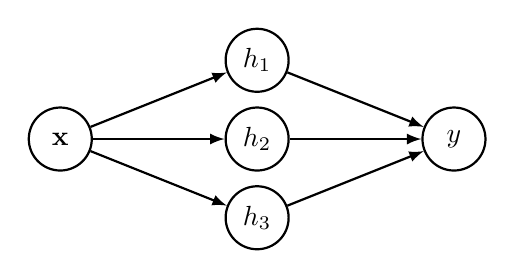
\begin{tikzpicture}[
                neuron/.style={circle,draw,thick,minimum size=8mm},
                connection/.style={-latex,thick},
                layer/.style={draw,rectangle,minimum height=15mm,minimum width=1.5cm,align=center},
            ]

            \node[neuron] (input) at (0,-2) {$\mathbf{x}$};

            \foreach \i in {1,...,3} {
                \node[neuron] (hidden\i) at (2.5,-\i) {$h_{\i}$};
            }

            \node[neuron] (output) at (5,-2) {$y$};

            \foreach \i in {1,...,3} {
                \draw[connection] (input) -- (hidden\i);
                \draw[connection] (hidden\i) -- (output);
            }
        \end{tikzpicture}
        \caption{Neural Network Architecture for the given regression problem}
        \label{fig:nn}
    \end{figure}
    The bias term for the hidden layer and for the output layer is $h$ and $b$ respectively.
    Let us assume the inital weights as follows:
    \begin{equation*}
        W_{1} = \begin{bmatrix}
            w_{11} & w_{12} & w_{13}
        \end{bmatrix}_{1 \times 3} = \begin{bmatrix}
            1.0 & 1.0 & 1.0
        \end{bmatrix} \text{ and }
        W_{2} = \begin{bmatrix}
            w_{21} \\ w_{22} \\ w_{23}
        \end{bmatrix}_{3 \times 1} = \begin{bmatrix}
            1.0 \\ 1.0 \\ 1.0
        \end{bmatrix}
    \end{equation*}
    The bias terms are initialized to zero. We use ReLU activation with a learning rate of $\eta = 0.1$.
    The given dataset is
    \begin{equation*}
        \mathbf{x} = \begin{bmatrix}
            1.2 \\ 0.8 \\ 2.0
        \end{bmatrix}_{3 \times 1} \text{ and } \mathbf{y} = \begin{bmatrix}
            y_{1} \\ y_{2} \\ y_{3}
        \end{bmatrix} = \begin{bmatrix}
            3.0 \\ 2.5 \\ 4.0
        \end{bmatrix}_{3 \times 1}
    \end{equation*}

    \subsubsection*{Iteration \#1 (Forward Pass)}
    For the first forward pass, we have ($A_{1}$ denotes $ReLU(Z_{1})$)
    \begin{align}
        Z_{1} = \mathbf{x} W_{1} + h &= \begin{bmatrix}
            1.2 \\ 0.8 \\ 2.0
        \end{bmatrix} \begin{bmatrix}
            1.0 & 1.0 & 1.0
        \end{bmatrix} + \mathbf{0} = \begin{bmatrix}
            1.2 & 1.2 & 1.2 \\
            0.8 & 0.8 & 0.8 \\
            2.0 & 2.0 & 2.0
        \end{bmatrix}_{3 \times 3}\\
        \mathbf{y} = A_{1} W_{2} + b &= \begin{bmatrix}
            1.2 & 1.2 & 1.2 \\
            0.8 & 0.8 & 0.8 \\
            2.0 & 2.0 & 2.0
        \end{bmatrix} \begin{bmatrix}
            1.0 \\ 1.0 \\ 1.0
        \end{bmatrix} + \mathbf{0} = \begin{bmatrix}
            3.6 \\ 2.4 \\ 6.0
        \end{bmatrix}_{3 \times 1}
    \end{align}
    Clearly, $A_{2} = \text{ReLU}(\mathbf{y}) = \mathbf{y}$.

    \subsubsection*{Iteration \#1 (Loss)}
    We find the mean squared error loss for the first iteration is given by
    \begin{equation}
        \mathcal{L}(\mathbf{W}) = \frac{1}{3} \sum_{i=1}^{3} (\hat{y}_{i} - y_{i})^{2} = \frac{(3.6 - 3.0)^{2} + (2.4 - 2.5)^{2} + (6.0 - 4.0)^{2}}{3} = \frac{4.37}{3} = 1.4567
    \end{equation}

    \subsubsection*{Iteration \#1 (Backward Pass)}
    For the backward pass, we first find the gradient of the loss with respect to the output
    \begin{align*}
        \frac{\partial \mathcal{L}}{\partial \mathbf{y}} &= \frac{1}{3} \sum_{i=1}^{3} \frac{\partial}{\partial \mathbf{y}} (\hat{y}_{i} - y_{i})^{2} \\
        &= \frac{1}{3} \sum_{i=1}^{3} 2 (\hat{y}_{i} - y_{i}) \frac{\partial}{\partial \mathbf{y}} (\hat{y}_{i} - y_{i}) \\
        &= \frac{-2}{3} \begin{bmatrix}
            3.6 - 3.0 & 2.4 - 2.5 & 6.0 - 4.0
        \end{bmatrix} = \begin{bmatrix}
            0.4 & -0.06 & 1.34
        \end{bmatrix}
    \end{align*}
    Then, we find the gradients of the loss with respect to the output layer weights
    and bias. This is given by
    \begin{align*}
        \frac{\partial \mathcal{L}}{\partial W_{2}} &= \left( \frac{\partial \mathcal{L}}{\partial \mathbf{y}} \frac{\partial \mathbf{y}}{\partial W_{2}} \right)^{T} \\
        \frac{\partial \mathbf{y}}{\partial W_{2}} &= \frac{\partial}{\partial W_{2}} (A_{1} W_{2} + b) = A_{1}^{T}
    \end{align*}
    So, updated weights $W_{2}$ are
    \begin{align*}
        W_{2} &= W_{2} - \eta \frac{\partial \mathcal{L}}{\partial W_{2}} \\
        &= W_{2} - \eta \left( \begin{bmatrix}
            0.4 & -0.06 & 1.34
        \end{bmatrix} \begin{bmatrix}
            1.2 & 0.8 & 2.0 \\
            1.2 & 0.8 & 2.0 \\
            1.2 & 0.8 & 2.0
        \end{bmatrix} \right)^{T} = \begin{bmatrix}
            1.0 \\ 1.0 \\ 1.0
        \end{bmatrix} - 0.1 \begin{bmatrix}
            2.016 \\ 1.344 \\ 3.36
        \end{bmatrix} = \begin{bmatrix}
            0.7984 \\ 0.8656 \\ 0.6640
        \end{bmatrix}
    \end{align*}
    Next, we find the gradient of the loss with respect to the bias term
    \begin{align*}
        \frac{\partial \mathcal{L}}{\partial b} &= \left( \frac{\partial \mathcal{L}}{\partial \mathbf{y}}  \frac{\partial \mathbf{y}}{\partial b} \right)^{T} \\
        \frac{\partial \mathbf{y}}{\partial b} &= \frac{\partial}{\partial b} (A_{1} W_{2} + b) = \mathbf{1}
    \end{align*}
    So, the updated bias term becomes
    \begin{align*}
        b = b - \eta \frac{\partial \mathcal{L}}{\partial b} &= b - \eta \left( \begin{bmatrix}
            0.4 & -0.06 & 1.34
        \end{bmatrix} \begin{bmatrix}
            1 \\ 1 \\ 1
        \end{bmatrix} \right)^{T} = 0 - 0.1 * 1.68 = -0.168
    \end{align*}
    Next, we find the gradient of the loss with respect to the hidden layer weights. This is given by
    \begin{align*}
        \frac{\partial \mathcal{L}}{\partial W_{1}} &= \frac{\partial \mathcal{L}}{\partial \mathbf{y}} \frac{\partial \mathbf{y}}{\partial Z_{1}} \left( \frac{\partial Z_{1}}{\partial W_{1}} \right)^{T} \\
        \frac{\partial \mathbf{y}}{\partial Z_{1}} &= \frac{\partial}{\partial Z_{1}} (A_{1} W_{2} + b) = W_{2} \\
        \frac{\partial Z_{1}}{\partial W_{1}} &= \frac{\partial}{\partial W_{1}} (\mathbf{x} W_{1} + h) = \mathbf{x}
    \end{align*}
    So, the updated weights $W_{1}$ are
    \begin{align*}
        W_{1} = W_{1} - \eta \frac{\partial \mathcal{L}}{\partial W_{1}} &= W_{1} - \eta \left( \begin{bmatrix}
            0.4 & -0.06 & 1.34
        \end{bmatrix} \begin{bmatrix}
            0.7984 \\ 0.8656 \\ 0.6640
        \end{bmatrix} \right) \begin{bmatrix}
            1.2 & 0.8 & 2.0
        \end{bmatrix} \\
        &= \begin{bmatrix}
            1.0 & 1.0 & 1.0
        \end{bmatrix} - 0.1 \begin{bmatrix}
            1.389 & 0.925 & 2.314
        \end{bmatrix} = \begin{bmatrix}
            0.86 & 0.90 & 0.76
        \end{bmatrix}
    \end{align*}
    Finally, we find the gradient of the loss with respect to the bias term of the hidden layer.
    This is given by
    \begin{align*}
        \frac{\partial \mathcal{L}}{\partial h} &= \frac{\partial \mathcal{L}}{\partial \mathbf{y}} \frac{\partial \mathbf{y}}{\partial Z_{1}} \left( \frac{\partial Z_{1}}{\partial h} \right)^{T} \\
        \frac{\partial Z_{1}}{\partial h} &= \frac{\partial}{\partial h} (\mathbf{x} W_{1} + h) = \mathbf{1}
    \end{align*}
    So, the updated bias term $h$ is
    \begin{align*}
        h = h - \eta \frac{\partial \mathcal{L}}{\partial h} &= h - \eta \left( \begin{bmatrix}
            0.4 & -0.06 & 1.34
        \end{bmatrix} \begin{bmatrix}
            0.7984 \\ 0.8656 \\ 0.6640
        \end{bmatrix} \right) \begin{bmatrix}
            1
        \end{bmatrix} = 0 - 0.1 * 1.157 = -0.1157
    \end{align*}

    \subsection*{Solution 2 (2 marks)}
    To predict the class of point $\mathbf{x}$ through an SVM, we find the sign of the equation
    \begin{equation}
        \sum_{i=1}^{n} \alpha_{i} y_{i} K(\mathbf{x}_{i}, \mathbf{x}) + b
    \end{equation}
    where $K(\cdot, \cdot)$ is the kernel function. For a gaussian SVM, the kernel
    function is
    \begin{equation}
        K(\mathbf{u}, \mathbf{v}) = \exp\left( - \frac{\lVert \mathbf{u} - \mathbf{v} \rVert_{2}^{2}}{2 \sigma^{2}} \right)
    \end{equation}
    So, to predict the class of a new data point $\mathbf{x}$, we apply the following rule for its classification
    \begin{equation}
        \text{sign} \left( \sum_{i=1}^{n} \alpha_{i} y_{i} \exp\left( - \frac{\lVert \mathbf{x}_{i} - \mathbf{x} \rVert_{2}^{2}}{2 \sigma^{2}} \right) + b \right)
    \end{equation}

    \subsection*{Solution 3}
    \begin{table}[htbp]
        \centering
        \begin{tabular}{cc|c}
            \textsc{Index} & \textsc{Data Points} & \textsc{Label} \\
            \hline
            $\mathbf{x}_{1}$ & $(2, 3)$ & $\mathbf{+1}$ \\
            $\mathbf{x}_{2}$ & $(6, 7)$ & $\mathbf{-1}$ \\
            $\mathbf{x}_{3}$ & $(5, 6)$ & $\mathbf{-1}$ \\
            $\mathbf{x}_{4}$ & $(4, 1)$ & $\mathbf{+1}$ \\
            $\mathbf{x}_{5}$ & $(1, 1)$ & $\mathbf{+1}$ \\
            $\mathbf{x}_{6}$ & $(7, 8)$ & $\mathbf{-1}$ \\
        \end{tabular}
        \caption{Data points for Problem 3}
        \label{tab:prob3}
    \end{table}

    \subsubsection*{(a) (1 mark)}
    \subsubsection*{Solution}
    \textbf{Yes}, the points are clearly linearly separable. This is because a line
    (a 2-dimensional hyperplane) can separate the points into two classes. Empirically,
    the points with higher $x$ and $y$ values belong to the class $\mathbf{-1}$ and the points
    with lower $x$ and $y$ values belong to the class $\mathbf{+1}$. \\
    The linear separability can be seen in Figure \ref{fig:prob3}.
    \begin{figure}[htbp]
        \centering
        \includegraphics[width=0.5\textwidth]{../Assets/points.png}
        \caption{Data points in Problem 3}
        \label{fig:prob3}
    \end{figure}

    \subsubsection*{(b) (1 mark)}
    \subsubsection*{Solution}
    To find the optimal linear decision boundary for the given data points, we need to find
    the optimal hyperplane that maximizes the margin. Let the equation of the hyperplane be
    \begin{equation}
        \label{eq:hyperplane}
        \mathbf{w}^T \mathbf{x} + b = 0
    \end{equation}
    where $\mathbf{w}$ is the normal vector to the hyperplane and $b$ is the bias term. The
    weights for the normal vector and bias are found by solving the following optimization problem
    \begin{equation}
        \label{eq:opt}
        \min_{\mathbf{w}, b} \ \frac{1}{2} \lVert \mathbf{w} \rVert_{2}^{2} \quad \text{subject to}
        \quad y_{i} (\mathbf{w}^T \mathbf{x}_{i} + b) \geq 1 \quad \forall \ i = 1, 2, \dots, 6
    \end{equation}
    To solve this, we solve its Lagrangian dual, which is
    \begin{align}
        \label{eq:dual}
        \max_{\alpha} L(\alpha) &= \sum_{i=1}^{6} \alpha_{i} - \frac{1}{2} \sum_{i=1}^{6} \sum_{j=1}^{6}
        y_{i} \alpha_{i} (\mathbf{x}_{i}^T \mathbf{x}_{j}) y_{j} \alpha_{j} \\
        \text{subject to} &\quad \sum_{i=1}^{6} \alpha_{i} y_{i} = 0 \quad \text{and} \quad \alpha_{i} \geq 0
        \quad \forall \ i = 1, 2, \dots, 6 \nonumber
    \end{align}
    To find the Lagrangian multipliers, we take the partial derivatives of the Lagrangian dual
    with respect to each $\alpha_{i}$ and set them to zero. This gives us
    \begin{equation}
        \label{eq:partial}
        \frac{\partial L}{\partial \alpha_{i}} = 1 - \frac{1}{2} \sum_{j=1}^{6} y_{i} (\mathbf{x}_{i}^T \mathbf{x}_{j}) y_{j} \alpha_{j} = 0
        \quad \forall \ i = 1, 2, \dots, 6
    \end{equation}
    Solving the system of these 6 linear equations, we get
    \begin{equation}
        \label{eq:optimal}
        \mathbf{w} = \begin{bmatrix} 1 \\ 1 \end{bmatrix} \quad \text{and} \quad b = -8 \quad
        \text{i.e.} \quad \mathbf{x}^{(1)} + \mathbf{x}^{(2)} - 8 = 0
    \end{equation}
    In the normalized form, the equation becomes
    \begin{equation}
        \label{eq:optimal-norm}
        \mathbf{w} = \frac{1}{\sqrt{2}} \begin{bmatrix} 1 \\ 1 \end{bmatrix} \quad \text{and} \quad b = -\frac{8}{\sqrt{2}} = -4 \sqrt{2} \quad
        \text{i.e.} \quad \frac{1}{\sqrt{2}}\mathbf{x}^{(1)} + \frac{1}{\sqrt{2}}\mathbf{x}^{(2)} - 4\sqrt{2} = 0
    \end{equation}
    A graph of the complete solution is given in Figure \ref{fig:prob3-sol}.
    \begin{figure}[htbp]
        \centering
        \includegraphics[width=0.5\textwidth]{../Assets/svs.png}
        \caption{Solution to Problem 3}
        \label{fig:prob3-sol}
    \end{figure}

    \subsubsection*{(c) (1 mark)}
    The data points $\mathbf{x}^{*}$ closest to the separating hyperplane, i.e.
    the support vectors are given in Table \ref{tab:support-vectors}. Note how the
    point $\mathbf{x}_{4} = (4, 1)$ is not a support vector even though it
    is the same distance from the hyperplane.
    \begin{table}[htbp]
        \centering
        \begin{tabular}{cc|c}
            \textsc{Index} & \textsc{Support Vectors} & \textsc{Label} \\
            \hline
            $\mathbf{x}_{1}$ & $(2, 3)$ & $\mathbf{+1}$ \\
            $\mathbf{x}_{3}$ & $(5, 6)$ & $\mathbf{-1}$ \\
        \end{tabular}
        \caption{Support Vectors for Data in Table \ref{tab:prob3}}
        \label{tab:support-vectors}
    \end{table}

    \subsubsection*{(d) (1 mark)}
    The margin of the decision boundary is given by substituting the support vectors
    in the equation
    \begin{align}
        \label{eq:margin}
        \gamma &= y^{*} \ \left( \frac{1}{\lVert \mathbf{w} \rVert_{2}} \left( \mathbf{w}^T \mathbf{x}^{*} + b \right) \right) \\
        &= -1 \left[ \frac{1}{\sqrt{2}} (1 \times 2 + 1 \times 3 - 8) \right] = \frac{3}{\sqrt{2}} = \frac{3\sqrt{2}}{2} \nonumber
    \end{align}
    Evidently, this is the distance between the hyperplane and the support vectors. The
    same value for $\gamma$ can be obtained by substituting the other support vector in the equation.
    Hence, the single margin is $\frac{3\sqrt{2}}{2}$ and the total margin is $3\sqrt{2}$.

    \subsubsection*{(e) (1 mark)}
    Clearly, the optimal margin will shift if we remove any support vector. For example,
    if we remove any support vector. If we remove $\mathbf{x}_{1}$, then empiraically,
    the slope of the separating hyperplane will decrease, and if we remove $\mathbf{x}_{2}$,
    then its slope increases.

    \section{Section B (Scratch Implementation)}
    In this section, we implemented a neural network from scratch using \texttt{numpy} package
    that meets certain requirements. The implementation can be found in \texttt{utils.py}. The
    implemented neural network was then tested on the MNIST dataset. The code for the solution
    can be found in the \texttt{main.ipynb} notebook.

    \subsection*{Activation Functions}
    One can use sigmoid, tanh, ReLU, Leaky ReLU, and Linear as the activation functions for the
    neural network by passing in the \texttt{activation} parameter. The softmax activation function
    is used in the last layer.

    \subsection*{Weight Initialization}
    The weights of the network can be initialized to three modes - random, normal, and zero,
    using the \texttt{weight\_init} parameter.

    \subsection*{Trained Neural Network}
    The neural network is trained to solve the MNSIT classification problem. The hidden layers are
    set to sizes $[256, 128, 64, 32]$. The plots for accuracies and losses per epoch are
    given in the notebook. The sigmoid activation function was found to give the best model.

    \section{Section C (Algorithm Implementation using Packages)}
    In this section, we use the \texttt{MLPClassifier} from the \texttt{sklearn} package to
    train a neural network on the SVHN dataset.

    \subsection*{Data Preparation}
    The dataset was downloaded from the given link, and split into a ratio of 70\% training,
    20\% validation, and 10\% testing. Some data visualization was also performed, and can be found
    in the same notebook.

    \subsection*{Model Training and Activation Functions}
    The neural network was trained with 2 hidden layers. The \texttt{GridSearchCV} function was
    to find the optimal hyperparameters for the netowrk. The ReLU activation function was found
    to be the best. Other optimal hyperparameters are given in table \ref{tab:hyperparams}.
    \begin{table}[htbp]
        \centering
        \begin{tabular}{c|c}
            \textsc{Hyperparameter} & \textsc{Value} \\
            \hline
            \texttt{activation} & \texttt{relu} \\
            \texttt{alpha} (learning-rate) & $0.05$ \\
            \texttt{batch\_size} & $250$ \\
            \texttt{hidden\_layer\_sizes} & $(128, 128)$
        \end{tabular}
        \caption{Optimal hyperparameters for the given neural network classifier}
        \label{tab:hyperparams}
    \end{table}

    \subsection*{Incorrect Predictions}
    The best model achieved a score of over 0.803. Some incorrect predictions from each class
    were visualized and their reasons were noted down. The observations are given in the
    same notebook.

    \section*{References}
    \begin{enumerate}
        \item \href{https://web.mit.edu/6.034/wwwbob/svm-notes-long-08.pdf}{\color{blue}\underline{An Idiot's Guide to Support Vector Machines}}
        \item \href{https://scikit-learn.org/stable/modules/generated/sklearn.neural_network.MLPClassifier.html}{\color{blue}\underline{\texttt{MLPClassifier} in Sci-kit Learn (Official Documentation)}}
    \end{enumerate}

\end{document}